% Select document class
\documentclass[aspectratio=169]{beamer}

% =============================================================================
% COMMON PREAMBLE (Assuming your network_preamble.tex handles standard packages)
% =============================================================================
% =============================================================================
% Common Preamble for Network+ Lecture Series
% This file provides consistent formatting, colors, packages, and styles
% across all lecture modules for both beamer presentations and article mode
% =============================================================================

% =============================================================================
% THEME AND COLORS
% =============================================================================
\usetheme{Madrid}
\usecolortheme{whale}

% Custom colors - standardized across all lectures
\definecolor{rctcblue}{RGB}{0, 74, 136}
\definecolor{rctcgold}{RGB}{255, 199, 44}
\definecolor{networkgreen}{RGB}{0, 128, 64}
\definecolor{alertred}{RGB}{180, 0, 0}
\definecolor{aborange}{RGB}{230, 126, 34}
\definecolor{copperbrown}{RGB}{184, 115, 51}
\definecolor{faborange}{RGB}{255, 165, 0}
\definecolor{fiberyellow}{RGB}{255, 215, 0}
\definecolor{shirepurple}{RGB}{102, 51, 153}
\definecolor{ipblue}{RGB}{52, 152, 219}
\definecolor{ippurple}{RGB}{155, 89, 182}
\definecolor{vlangreen}{RGB}{39, 174, 96}
\definecolor{tcpblue}{RGB}{30, 100, 180}
\definecolor{udpgreen}{RGB}{50, 160, 80}
\definecolor{dhcppurple}{RGB}{120, 60, 160}
\definecolor{dnsyellow}{RGB}{200, 170, 50}
\definecolor{batblack}{RGB}{30, 30, 40}
\definecolor{gothamgray}{RGB}{80, 85, 95}
\definecolor{paddysgreen}{RGB}{19, 77, 33}
\definecolor{beerlight}{RGB}{255, 199, 44}
\definecolor{sunnyorange}{RGB}{255, 140, 0}
\definecolor{ogregreen}{RGB}{34, 139, 34}
\definecolor{swampbrown}{RGB}{101, 67, 33}

% Set theme colors
\setbeamercolor{palette primary}{bg=rctcblue,fg=white}
\setbeamercolor{palette secondary}{bg=rctcblue!80,fg=white}
\setbeamercolor{palette tertiary}{bg=rctcblue!60,fg=white}
\setbeamercolor{structure}{fg=rctcblue}
\setbeamercolor{title}{fg=white,bg=rctcblue}
\setbeamercolor{frametitle}{fg=white,bg=rctcblue}
\setbeamercolor{block title}{bg=rctcblue,fg=white}
\setbeamercolor{block body}{bg=rctcblue!10,fg=black}
\setbeamercolor{block title alerted}{bg=alertred,fg=white}
\setbeamercolor{block body alerted}{bg=alertred!10,fg=black}
\setbeamercolor{block title example}{bg=networkgreen,fg=white}
\setbeamercolor{block body example}{bg=networkgreen!10,fg=black}

% =============================================================================
% PACKAGES
% =============================================================================
\usepackage[utf8]{inputenc}
\usepackage[T1]{fontenc}
\usepackage{lmodern}  % Better font rendering
\usepackage{graphicx}
\usepackage{tikz}
\usepackage{booktabs}
\usepackage{array}
\usepackage{multirow}
\usepackage{hyperref}
\usepackage{adjustbox}
\usepackage{amssymb}
\usepackage{amsmath}
\usepackage{calc}
\usepackage{fontawesome5}
% xcolor with [table] option: avoid colortbl.4ht hook conflict in tex4ht
\ifdefined\HCode
  \usepackage{xcolor}
  \usepackage{colortbl}  % provides \rowcolor etc.
\else
  \usepackage[table]{xcolor}  % includes colortbl for pdflatex
\fi

% =============================================================================
% TIKZ LIBRARIES AND SETUP
% =============================================================================
\usetikzlibrary{
    shapes.geometric,
    shapes.symbols,
    shapes.misc,
    arrows.meta,
    positioning,
    calc,
    fit,
    backgrounds,
    decorations.pathreplacing,
    decorations.pathmorphing,
    matrix,
    chains
}
% shadows library causes pgfuseshading errors with tex4ht;
% only load it when NOT building HTML
\ifdefined\HCode\else
    \usetikzlibrary{shadows}
\fi

% Graphics path for icons and chapter images
\graphicspath{
    {../images/icons/}
    {./images/icons/}
    {images/icons/}
    {../images/ch1/}
    {./images/ch1/}
    {images/ch1/}
    {../images/ch2/}
    {./images/ch2/}
    {images/ch2/}
    {../images/ch3/}
    {./images/ch3/}
    {images/ch3/}
    {../images/ch4/}
    {./images/ch4/}
    {images/ch4/}
    {../images/ch5/}
    {./images/ch5/}
    {images/ch5/}
    {../images/ch6/}
    {./images/ch6/}
    {images/ch6/}
    {../images/ch7/}
    {./images/ch7/}
    {images/ch7/}
    {../images/ch8/}
    {./images/ch8/}
    {images/ch8/}
    {../images/ch9/}
    {./images/ch9/}
    {images/ch9/}
    {../images/}
    {./images/}
    {images/}
}

% =============================================================================
% NETWORK DIAGRAM STYLES
% =============================================================================
\tikzset{
    % Node styles for network devices
    device/.style={
        inner sep=2pt,
        label distance=2pt
    },
    pc/.style={device},
    laptop/.style={device},
    server/.style={device},
    router/.style={device},
    switch/.style={device},
    firewall/.style={device},
    cloud/.style={device},
    phone/.style={device},
    tablet/.style={device},
    wifi/.style={device},
    % Connection styles
    ethernet/.style={
        draw=rctcblue,
        line width=1.5pt,
        -{Stealth[length=3mm]}
    },
    ethernet noarrow/.style={
        draw=rctcblue,
        line width=1.5pt
    },
    wireless/.style={
        draw=aborange,
        line width=1.5pt,
        dashed,
        -{Stealth[length=3mm]}
    },
    wireless noarrow/.style={
        draw=aborange,
        line width=1.5pt,
        dashed
    },
    wan/.style={
        draw=alertred,
        line width=2pt,
        -{Stealth[length=3mm]}
    },
    wan noarrow/.style={
        draw=alertred,
        line width=2pt
    },
    copper/.style={
        draw=copperbrown,
        line width=2pt,
        -{Stealth[length=3mm]}
    },
    copper noarrow/.style={
        draw=copperbrown,
        line width=2pt
    },
    fiber/.style={
        draw=fiberyellow,
        line width=2pt,
        -{Stealth[length=3mm]}
    },
    fiber noarrow/.style={
        draw=fiberyellow,
        line width=2pt
    },
    trunk/.style={
        draw=shirepurple,
        line width=2pt,
        -{Stealth[length=3mm]}
    },
    trunk noarrow/.style={
        draw=shirepurple,
        line width=2pt
    },
    % Packet/segment styles
    pktseg/.style={
        draw=rctcblue,
        fill=rctcblue!10,
        minimum height=0.5cm,
        font=\tiny,
        rounded corners=2pt
    },
    pktseg tcp/.style={
        draw=tcpblue,
        fill=tcpblue!15,
        minimum height=0.5cm,
        font=\tiny,
        rounded corners=2pt
    },
    pktseg udp/.style={
        draw=udpgreen,
        fill=udpgreen!15,
        minimum height=0.5cm,
        font=\tiny,
        rounded corners=2pt
    },
    pktseg highlight/.style={
        draw=aborange,
        fill=aborange!20,
        minimum height=0.5cm,
        font=\tiny,
        rounded corners=2pt
    },
    % Box styles
    ipbox/.style={
        draw=rctcblue,
        fill=rctcblue!10,
        rounded corners,
        minimum height=0.4cm,
        font=\small
    },
    portbox/.style={
        draw=tcpblue,
        fill=tcpblue!10,
        rounded corners,
        minimum height=0.4cm,
        font=\small
    },
    dnsbox/.style={
        draw=dnsyellow,
        fill=dnsyellow!15,
        rounded corners,
        minimum height=0.4cm,
        font=\small
    },
    routetable/.style={
        draw=rctcblue,
        fill=rctcblue!10,
        rounded corners,
        minimum height=0.4cm,
        font=\small
    },
    macbox/.style={
        draw=networkgreen,
        fill=networkgreen!10,
        rounded corners,
        minimum height=0.4cm,
        font=\small
    },
    % Frame segment styles (Ethernet frame diagrams)
    frameseg/.style={
        draw=rctcblue,
        fill=rctcblue!10,
        minimum height=0.5cm,
        font=\tiny,
        rounded corners=2pt
    },
    frameseg highlight/.style={
        draw=aborange,
        fill=aborange!20,
        minimum height=0.5cm,
        font=\tiny,
        rounded corners=2pt
    },
    % Process/flow styles
    process/.style={
        draw=rctcblue,
        fill=rctcblue!15,
        rounded corners,
        minimum width=2cm,
        minimum height=0.6cm,
        font=\small,
        align=center
    },
    decision/.style={
        draw=aborange,
        fill=aborange!15,
        diamond,
        aspect=2,
        minimum width=1.5cm,
        font=\small,
        align=center
    },
    % OSI Layer styles
    osilayer/.style={
        draw=rctcblue,
        fill=rctcblue!10,
        minimum width=3cm,
        minimum height=0.45cm,
        font=\small
    },
    osilayer highlight/.style={
        draw=aborange,
        fill=aborange!20,
        line width=1.5pt,
        minimum width=3cm,
        minimum height=0.45cm,
        font=\small\bfseries
    }
}

% =============================================================================
% ICON COMMANDS - Standardized using PNG files and FontAwesome
% =============================================================================
% Network device icons (PNG)
\newcommand{\iconpc}[1][0.6cm]{\resizebox{#1}{!}{
\includegraphics{icon_pc}}}
\newcommand{\iconlaptop}[1][0.6cm]{\resizebox{#1}{!}{
\includegraphics{icon_laptop}}}
\newcommand{\iconserver}[1][0.6cm]{\resizebox{#1}{!}{
\includegraphics{icon_server}}}
\newcommand{\iconrouter}[1][0.6cm]{\resizebox{#1}{!}{
\includegraphics{icon_router}}}
\newcommand{\iconswitch}[1][0.6cm]{\resizebox{#1}{!}{
\includegraphics{icon_switch}}}
\newcommand{\iconfirewall}[1][0.6cm]{\resizebox{#1}{!}{
\includegraphics{icon_firewall}}}
\newcommand{\iconcloud}[1][0.6cm]{\resizebox{#1}{!}{
\includegraphics{icon_cloud}}}
\newcommand{\iconphone}[1][0.6cm]{\resizebox{#1}{!}{
\includegraphics{icon_phone}}}
\newcommand{\icontablet}[1][0.6cm]{\resizebox{#1}{!}{
\includegraphics{icon_tablet}}}
\newcommand{\iconwifi}[1][0.6cm]{\resizebox{#1}{!}{
\includegraphics{icon_wifi}}}
\newcommand{\icondatabase}[1][0.6cm]{\resizebox{#1}{!}{
\includegraphics{icon_db}}}
\newcommand{\iconlock}[1][0.6cm]{\resizebox{#1}{!}{
\includegraphics{icon_lock}}}

% For HTML/tex4ht builds: replace PNG icons with FontAwesome5 glyphs.
% dvisvgm embeds font glyphs as vectors but silently ignores em:graph (PNG)
% specials, so PNG icons would be blank in the output SVGs. FA5 glyphs work.
\ifdefined\HCode
  \renewcommand{\iconpc}[1][0.6cm]{\resizebox{#1}{!}{\faIcon{desktop}}}
  \renewcommand{\iconlaptop}[1][0.6cm]{\resizebox{#1}{!}{\faIcon{laptop}}}
  \renewcommand{\iconserver}[1][0.6cm]{\resizebox{#1}{!}{\faIcon{server}}}
  \renewcommand{\iconrouter}[1][0.6cm]{\resizebox{#1}{!}{\faIcon{route}}}
  \renewcommand{\iconswitch}[1][0.6cm]{\resizebox{#1}{!}{\faIcon{network-wired}}}
  \renewcommand{\iconfirewall}[1][0.6cm]{\resizebox{#1}{!}{\faIcon{shield-alt}}}
  \renewcommand{\iconcloud}[1][0.6cm]{\resizebox{#1}{!}{\faIcon{cloud}}}
  \renewcommand{\iconphone}[1][0.6cm]{\resizebox{#1}{!}{\faIcon{mobile-alt}}}
  \renewcommand{\icontablet}[1][0.6cm]{\resizebox{#1}{!}{\faIcon{tablet-alt}}}
  \renewcommand{\iconwifi}[1][0.6cm]{\resizebox{#1}{!}{\faIcon{wifi}}}
  \renewcommand{\icondatabase}[1][0.6cm]{\resizebox{#1}{!}{\faIcon{database}}}
  \renewcommand{\iconlock}[1][0.6cm]{\resizebox{#1}{!}{\faIcon{lock}}}
\fi

% FontAwesome icons
\newcommand{\iconuser}[1][0.6cm]{\resizebox{#1}{!}{\faIcon{user}}}
\newcommand{\iconglobe}[1][0.6cm]{\resizebox{#1}{!}{\faIcon{globe}}}
\newcommand{\iconclock}[1][0.6cm]{\resizebox{#1}{!}{\faIcon{clock}}}
\newcommand{\iconmail}[1][0.6cm]{\resizebox{#1}{!}{\faIcon{envelope}}}
\newcommand{\icondoc}[1][0.6cm]{\resizebox{#1}{!}{\faIcon{file-alt}}}
\newcommand{\iconsearch}[1][0.6cm]{\resizebox{#1}{!}{\faIcon{search}}}
\newcommand{\icontools}[1][0.6cm]{\resizebox{#1}{!}{\faIcon{tools}}}
\newcommand{\iconchart}[1][0.6cm]{\resizebox{#1}{!}{\faIcon{chart-line}}}
\newcommand{\iconalert}[1][0.6cm]{\resizebox{#1}{!}{\faIcon{bell}}}
\newcommand{\iconlog}[1][0.6cm]{\resizebox{#1}{!}{\faIcon{clipboard-list}}}
\newcommand{\iconeye}[1][0.6cm]{\resizebox{#1}{!}{\faIcon{eye}}}
\newcommand{\iconhacker}[1][0.6cm]{\resizebox{#1}{!}{\faIcon{user-secret}}}
\newcommand{\iconkey}[1][0.6cm]{\resizebox{#1}{!}{\faIcon{key}}}
\newcommand{\iconfile}[1][0.6cm]{\resizebox{#1}{!}{\faIcon{file-alt}}}
\newcommand{\icondog}[1][0.6cm]{\resizebox{#1}{!}{\faIcon{dog}}}
\newcommand{\iconcat}[1][0.6cm]{\resizebox{#1}{!}{\faIcon{cat}}}
\newcommand{\iconvoip}[1][0.6cm]{\resizebox{#1}{!}{\faIcon{phone-volume}}}
\newcommand{\iconmoney}[1][0.6cm]{\resizebox{#1}{!}{\faIcon{money-bill-wave}}}
\newcommand{\icontrash}[1][0.6cm]{\resizebox{#1}{!}{\faIcon{trash}}}
\newcommand{\iconbuilding}[1][0.6cm]{\resizebox{#1}{!}{\faIcon{building}}}

% =============================================================================
% CUSTOM COMMANDS AND ENVIRONMENTS
% =============================================================================

% Key term formatting
\newcommand{\keyterm}[1]{\textbf{#1}}

% Slide section marker
\newcommand{\sectionslide}[1]{
    \begin{frame}
        \vfill
        \centering
        \begin{beamercolorbox}[sep=8pt,center,shadow=true,rounded=true]{title}
            \usebeamerfont{title}\Huge #1
        \end{beamercolorbox}
        \vfill
    \end{frame}
}

% Case study frame environment
\newenvironment{casestudy}[1]{%
    \begin{alertblock}{$\blacktriangleright$ Case Study: #1}
}{%
    \end{alertblock}
}

% Solution frame environment  
\newenvironment{casesolution}[1]{%
    \begin{exampleblock}{$\checkmark$ Solution: #1}
}{%
    \end{exampleblock}
}

% =============================================================================
% FOOTER WITH SLIDE NUMBERS
% =============================================================================
\setbeamertemplate{footline}{
    \leavevmode%
    \hbox{%
        \begin{beamercolorbox}[wd=.333333\paperwidth,ht=2.25ex,dp=1ex,center]{author in head/foot}%
            \usebeamerfont{author in head/foot}\insertshortauthor
        \end{beamercolorbox}%
        \begin{beamercolorbox}[wd=.333333\paperwidth,ht=2.25ex,dp=1ex,center]{title in head/foot}%
            \usebeamerfont{title in head/foot}\insertshorttitle
        \end{beamercolorbox}%
        \begin{beamercolorbox}[wd=.333333\paperwidth,ht=2.25ex,dp=1ex,right]{date in head/foot}%
            \usebeamerfont{date in head/foot}\insertshortdate{}\hspace*{2em}
            \insertframenumber{} / \inserttotalframenumber\hspace*{2ex}
        \end{beamercolorbox}}%
    \vskip0pt%
}

% =============================================================================
% ARTICLE MODE SUPPORT
% =============================================================================
% The following commands help with beamerarticle mode for HTML conversion

% In article mode, add proper section/subsection support and override environments
\mode<article>{
    % Make sure figure captions work properly
    \setbeamertemplate{caption}[numbered]
    \setbeamertemplate{caption label separator}{: }
    
    % Add some spacing for readability
    \setlength{\parskip}{0.5em}
    \setlength{\parindent}{0pt}
    
    % Article mode versions of case study environments
    \renewenvironment{casestudy}[1]{%
        \vspace{0.3cm}\noindent\textbf{Case Study: #1}\newline\begin{itshape}
    }{%
        \end{itshape}\vspace{0.3cm}
    }
    
    \renewenvironment{casesolution}[1]{%
        \vspace{0.3cm}\noindent\textbf{Solution: #1}\newline\begin{itshape}
    }{%
        \end{itshape}\vspace{0.3cm}
    }
}

% Command to mark content that only appears in article mode
\newcommand{\articleonly}[1]{\mode<article>{#1}}

% Command to mark content that only appears in presentation mode
\newcommand{\presentationonly}[1]{\mode<presentation>{#1}}


% Additional TikZ styles specific to this lecture
\tikzset{
    boxstyle/.style={
        rectangle,
        draw=rctcblue,
        fill=rctcblue!10,
        rounded corners=3pt,
        minimum width=2cm,
        minimum height=0.6cm,
        font=\small
    },
    process/.style={
        rectangle,
        draw=rctcblue,
        fill=rctcblue!20,
        text width=2.5cm,
        text centered,
        rounded corners,
        minimum height=0.8cm,
        font=\scriptsize\bfseries
    },
    decision/.style={
        diamond,
        draw=networkgreen,
        fill=networkgreen!20,
        text width=1.5cm,
        text centered,
        minimum height=1cm,
        font=\scriptsize\bfseries
    },
    channel curve/.style={
        thick,
        opacity=0.6
    }
}

% =============================================================================
% DOCUMENT INFO
% =============================================================================
\title{Wireless Networking Fundamentals}
\subtitle{Module 12.0 -- Deep Dive}
\author[B. Shea]{Brendan Shea, PhD}
\institute[RCTC]{Rochester Community and Technical College\\Intro to Networking}
\date{}

\begin{document}

% =============================================================================
% SLIDE 1: TITLE
% =============================================================================
\begin{frame}
    \titlepage
    \begin{center}
        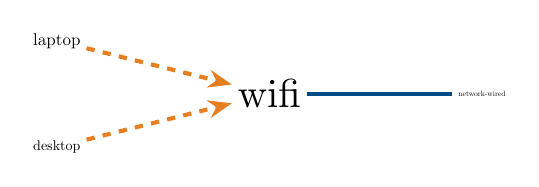
\begin{tikzpicture}[scale=0.9]
            % Simple wireless illustration for title
            \node[pc] (pc1) at (0,0) {\iconpc[0.6cm]};
            \node[laptop] (lap) at (0,1.5) {\iconlaptop[0.6cm]};
            \node[wifi] (ap) at (3,0.75) {\iconwifi[0.8cm]};
            \node[switch] (sw) at (6,0.75) {\iconswitch[0.6cm]};
            
            \draw[wireless] (pc1) -- (ap);
            \draw[wireless] (lap) -- (ap);
            \draw[ethernet noarrow] (ap) -- (sw);
        \end{tikzpicture}
    \end{center}
\end{frame}

% =============================================================================
% SLIDE 2: REVIEW
% =============================================================================
\begin{frame}{Review: From Wired to Wireless Physical Layers}
    \begin{columns}[T]
        \begin{column}{0.55\textwidth}
            \begin{itemize}
                \item \textbf{Layer 1 \& 2 Shift:} We are moving from IEEE \textbf{802.3 (Ethernet)} to IEEE \textbf{802.11 (WLAN)}.
                \item \textbf{Guided vs. Unguided Media:} Instead of voltages on copper or photons in glass fiber (guided), data is modulated onto electromagnetic waves broadcasted into open space (unguided).
                \item \textbf{Collision Domains:} A wired switch port is a collision domain of one (Full-Duplex). A wireless channel is a massive, shared collision domain (Half-Duplex) acting logically like a legacy Ethernet hub.
            \end{itemize}
        \end{column}
        \begin{column}{0.4\textwidth}
            \begin{alertblock}{The Core Challenge}
                In wired networks, the cable protects the signal. In wireless, the medium is hostile, shared, and constantly subject to physical interference and atmospheric degradation.
            \end{alertblock}
        \end{column}
    \end{columns}
\end{frame}

% =============================================================================
% SLIDE 3: LEARNING OUTCOMES
% =============================================================================
\begin{frame}{Learning Outcomes (Network+ Objectives)}
    Mapping directly to CompTIA Network+ domains, you will be able to:
    \vspace{0.5em}
    \begin{itemize}
        \item \textbf{Analyze} fundamental RF characteristics: frequency, amplitude, and phase modulation.
        \item \textbf{Calculate} the impact of overlapping vs. non-overlapping channels in 2.4GHz, 5GHz, and 6GHz bands.
        \item \textbf{Deconstruct} the CSMA/CA protocol, including the RTS/CTS mechanism for resolving the hidden node problem.
        \item \textbf{Differentiate} 802.11 iterations based on modulation techniques (DSSS, OFDM, OFDMA) and spatial streaming (MIMO).
        \item \textbf{Design} physical AP layouts utilizing appropriate antenna polarizations and radiation patterns (Omni vs. Yagi/Patch).
    \end{itemize}
\end{frame}

% =============================================================================
% SLIDE 4: SECTION 1 INTRO
% =============================================================================
\begin{frame}
    \begin{center}
        \Huge \textbf{Section 1}\\
        \vspace{0.5em}
        \Large \textcolor{rctcblue}{Basic Wireless Concepts}
    \end{center}
\end{frame}

% =============================================================================
% SLIDE 5: THE WIRELESS MEDIUM
% =============================================================================
\begin{frame}{The Wireless Medium: Radio Frequency (RF)}
    \begin{columns}[T]
        \begin{column}{0.55\textwidth}
            \begin{itemize}
                \item \textbf{Carrier Waves:} Access Points generate a continuous sine wave (the carrier). 
                \item \textbf{Modulation:} Data (1s and 0s) is superimposed onto the carrier wave by rapidly altering its state.
                \item \textbf{QAM (Quadrature Amplitude Modulation):} Modern Wi-Fi alters \emph{both} the phase and the amplitude simultaneously to encode multiple bits per symbol (e.g., 256-QAM or 1024-QAM).
                \item \textbf{Environmental Variables:} Unlike a Cat6 cable, an RF signal's SNR (Signal-to-Noise Ratio) constantly fluctuates based on moving physical objects and competing transmitters.
            \end{itemize}
        \end{column}
        \begin{column}{0.4\textwidth}
            \begin{block}{The Half-Duplex Reality}
                A wireless radio uses the exact same antenna to transmit and receive. It cannot do both at once without deafening itself. 
                \\ \vspace{0.5em}
                Therefore, \textbf{all Wi-Fi is strictly half-duplex}.
            \end{block}
        \end{column}
    \end{columns}
\end{frame}

% =============================================================================
% SLIDE 6: RF CHARACTERISTICS
% =============================================================================
\begin{frame}{RF Characteristics: Frequency, Wavelength, and Amplitude}
    \begin{itemize}
        \item \textbf{Frequency ($f$):} The number of full wave cycles per second, measured in Hertz (Hz). Wi-Fi operates in the Gigahertz (GHz) range (billions of cycles per second).
        \item \textbf{Wavelength ($\lambda$):} The physical distance between two consecutive peaks of a wave.
    \end{itemize}
    
    \begin{columns}[T]
        \begin{column}{0.5\textwidth}
            \begin{alertblock}{The Speed of Light Equation}
                $c = \lambda f$ \\
                \vspace{0.5em}
                \scriptsize Because the speed of light ($c$) is constant, frequency and wavelength are inversely related. As frequency increases, wavelength gets shorter.
            \end{alertblock}
        \end{column}
        \begin{column}{0.45\textwidth}
            \begin{itemize}
                \item \textbf{Amplitude:} The power/strength of the wave, often measured in decibel-milliwatts (dBm). 
                \item Lower frequency (longer wavelength) waves penetrate solid objects much better than high-frequency waves.
            \end{itemize}
        \end{column}
    \end{columns}
\end{frame}

% =============================================================================
% SLIDE 7: 2.4 vs 5 GHz
% =============================================================================
\begin{frame}{The 2.4 GHz vs. 5 GHz Bands}
    \begin{table}[]
        \renewcommand{\arraystretch}{1.5}
        \centering
        \small
        \begin{tabular}{|p{2.5cm}|p{5.5cm}|p{5.5cm}|}
        \hline
        \rowcolor[HTML]{EFEFEF} \textbf{Metric} & \textbf{2.4 GHz ISM Band} & \textbf{5 GHz UNII Bands} \\ \hline
        \textbf{Wavelength} & $\approx 4.9$ inches (Longer) & $\approx 2.3$ inches (Shorter) \\ \hline
        \textbf{Attenuation} & Excellent at penetrating drywall, brick, and wood. & Absorbed quickly by walls; heavily attenuated by water. \\ \hline
        \textbf{Capacity} & Only 3 non-overlapping channels (1, 6, 11). & Up to 24 non-overlapping 20MHz channels. \\ \hline
        \textbf{Interference} & Highly congested (Microwaves, Bluetooth, IoT, neighbors). & Relatively clean, though some channels require DFS (radar avoidance). \\ \hline
        \textbf{Max Throughput} & Low (Usually constrained to 20MHz widths). & High (Supports 40MHz, 80MHz, and 160MHz channel bonding). \\ \hline
        \end{tabular}
    \end{table}
\end{frame}

% =============================================================================
% SLIDE 8: 6 GHz
% =============================================================================
\begin{frame}{The New Frontier: 6 GHz and Wi-Fi 6E/7}
    \begin{columns}[T]
        \begin{column}{0.5\textwidth}
            \begin{itemize}
                \item \textbf{The Spectrum Starvation Problem:} Enterprise 5 GHz networks ran out of space when trying to bond channels for higher gigabit speeds.
                \item \textbf{The 6 GHz Solution:} The FCC opened 1,200 MHz of entirely new, contiguous spectrum for Wi-Fi 6E and Wi-Fi 7.
                \item Yields \textbf{59} new 20 MHz channels, or 7 massive 160 MHz channels.
            \end{itemize}
        \end{column}
        \begin{column}{0.48\textwidth}
            \begin{block}{Greenfield Deployment}
                Unlike 2.4/5 GHz, the 6 GHz band strictly prohibits legacy standards (802.11a/b/g/n/ac). Only highly efficient 802.11ax/be devices are allowed.
                \\ \vspace{0.5em}
                \textbf{Security Constraint:} WPA3 is strictly mandatory on the 6 GHz band. You cannot configure an open or WPA2 6 GHz SSID.
            \end{block}
        \end{column}
    \end{columns}
\end{frame}

% =============================================================================
% SLIDE 9: CHANNELS
% =============================================================================
\begin{frame}{Channels and Co-Channel Interference}
    \begin{columns}[T]
        \begin{column}{0.5\textwidth}
            \begin{itemize}
                \item The 2.4GHz band is 72 MHz wide, divided into 11 channels (in the US).
                \item \textbf{The Math Problem:} Each 802.11 standard channel requires roughly 20-22 MHz of frequency space, but the channels are drawn only \textbf{5 MHz apart}.
                \item Therefore, Channel 2 physically overlaps with 1, 3, 4, and 5. 
                \item \textbf{CCI (Co-Channel):} APs on the exact same channel politely wait their turn.
                \item \textbf{ACI (Adjacent Channel):} APs on overlapping channels (e.g., 1 and 2) talk over each other as unintelligible RF noise, causing massive packet loss.
            \end{itemize}
        \end{column}
        \begin{column}{0.48\textwidth}
            \begin{center}
                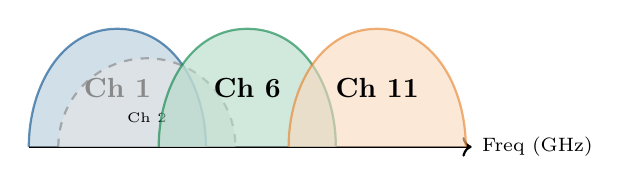
\begin{tikzpicture}[scale=0.75]
                    % Frequency line
                    \draw[thick, ->] (0,0) -- (7.5,0) node[right, font=\scriptsize] {Freq (GHz)};
                    
                    % Channel 1
                    \draw[fill=rctcblue!30, draw=rctcblue, channel curve] (0,0) to[out=90,in=180] (1.5,2) to[out=0,in=90] (3,0);
                    \node[font=\footnotesize, font=\bfseries] at (1.5, 1) {Ch 1};
                    
                    % Channel 2 (overlapping)
                    \draw[fill=gray!20, draw=gray, channel curve, dashed] (0.5,0) to[out=90,in=180] (2.0,1.5) to[out=0,in=90] (3.5,0);
                    \node[font=\tiny] at (2.0, 0.5) {Ch 2};
                    
                    % Channel 6
                    \draw[fill=networkgreen!30, draw=networkgreen, channel curve] (2.2,0) to[out=90,in=180] (3.7,2) to[out=0,in=90] (5.2,0);
                    \node[font=\footnotesize, font=\bfseries] at (3.7, 1) {Ch 6};
                    
                    % Channel 11
                    \draw[fill=aborange!30, draw=aborange, channel curve] (4.4,0) to[out=90,in=180] (5.9,2) to[out=0,in=90] (7.4,0);
                    \node[font=\footnotesize, font=\bfseries] at (5.9, 1) {Ch 11};
                \end{tikzpicture}
            \end{center}
            \vspace{0.2em}
            \begin{center}
                \scriptsize\parbox{0.92\linewidth}{\centering \textbf{2.4 GHz rule:}\\Use channels \textbf{1, 6, and 11} only.}
            \end{center}
        \end{column}
    \end{columns}
\end{frame}

% =============================================================================
% SLIDE 10: CSMA/CA
% =============================================================================
\begin{frame}{CSMA/CA \& The Hidden Node Problem}
    \begin{columns}[T]
        \begin{column}{0.48\textwidth}
            \begin{itemize}
                \item \textbf{CSMA/CA} relies on a Clear Channel Assessment (CCA).
                \item \textbf{Hidden Node Problem:} Laptop A and Laptop B can both reach the AP, but are too far apart to hear \emph{each other}. They might transmit simultaneously, causing a collision at the AP.
                \item \textbf{Solution (RTS/CTS):} Instead of just sending data, the device sends a tiny Request-To-Send. The AP replies with a Clear-To-Send, which tells \emph{all} other devices to set their Network Allocation Vector (NAV) timer and be quiet.
            \end{itemize}
        \end{column}
        \begin{column}{0.5\textwidth}
            \begin{center}
                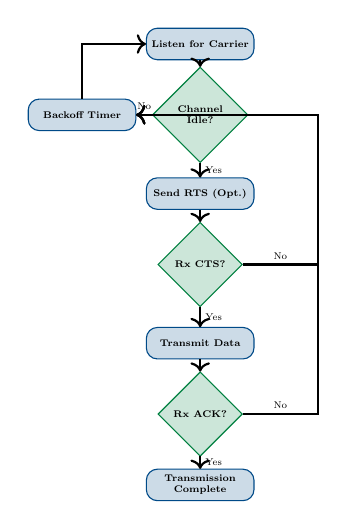
\begin{tikzpicture}[scale=0.50, every node/.style={transform shape}]
                    \node[process] (listen) at (0,0) {Listen for Carrier};
                    \node[decision] (idle) at (0,-1.8) {Channel Idle?};
                    \node[process] (wait) at (-3,-1.8) {Backoff Timer};
                    
                    \node[process] (rts) at (0,-3.8) {Send RTS (Opt.)};
                    \node[decision] (cts) at (0,-5.6) {Rx CTS?};
                    
                    \node[process] (send) at (0,-7.6) {Transmit Data};
                    \node[decision] (ack) at (0,-9.4) {Rx ACK?};
                    \node[process] (done) at (0,-11.2) {Transmission Complete};
                    
                    \draw[->, thick] (listen) -- (idle);
                    \draw[->, thick] (idle) -- node[above, font=\scriptsize] {No} (wait);
                    \draw[->, thick] (wait) |- (listen);
                    
                    \draw[->, thick] (idle) -- node[right, font=\scriptsize] {Yes} (rts);
                    \draw[->, thick] (rts) -- (cts);
                    
                    \draw[->, thick] (cts) -- node[above, font=\scriptsize] {No} (3,-5.6) |- (wait);
                    \draw[->, thick] (cts) -- node[right, font=\scriptsize] {Yes} (send);
                    
                    \draw[->, thick] (send) -- (ack);
                    \draw[->, thick] (ack) -- node[above, font=\scriptsize] {No} (3,-9.4) |- (wait);
                    \draw[->, thick] (ack) -- node[right, font=\scriptsize] {Yes} (done);
                \end{tikzpicture}
            \end{center}
        \end{column}
    \end{columns}
\end{frame}

% =============================================================================
% SLIDE 11: SECTION 2 INTRO
% =============================================================================
\begin{frame}
    \begin{center}
        \Huge \textbf{Section 2}\\
        \vspace{0.5em}
        \Large \textcolor{rctcblue}{Wireless Standards (802.11)}
    \end{center}
\end{frame}

% =============================================================================
% SLIDE 12: EVOLUTION OF WI-FI (TABLE)
% =============================================================================
\begin{frame}{The Evolution of Wi-Fi: Standards and Generations}
    \begin{itemize}
        \item The \keyterm{IEEE 802.11} working group defines the PHY (Physical) and MAC (Media Access Control) layers for wireless LANs.
        \item The \keyterm{Wi-Fi Alliance} introduced generational names (Wi-Fi 4, 5, 6) to simplify marketing and consumer understanding.
    \end{itemize}
    
    \vspace{0.3em}
    \begin{table}[]
        \renewcommand{\arraystretch}{1.4}
        \centering
        \scriptsize
        \resizebox{\textwidth}{!}{%
        \begin{tabular}{|l|l|l|l|l|}
        \hline
        \rowcolor[HTML]{EFEFEF} \textbf{IEEE Standard} & \textbf{Wi-Fi Name} & \textbf{Frequency Band(s)} & \textbf{Max Theo. Speed} & \textbf{Key Physical Innovation} \\ \hline
        \textbf{802.11b} (1999) & Wi-Fi 1 & 2.4 GHz & 11 Mbps & DSSS (Direct Sequence Spread Spectrum) \\ \hline
        \textbf{802.11a} (1999) & Wi-Fi 2 & 5 GHz & 54 Mbps & OFDM (Orthogonal Frequency Division) \\ \hline
        \textbf{802.11g} (2003) & Wi-Fi 3 & 2.4 GHz & 54 Mbps & Brought OFDM to the 2.4 GHz band \\ \hline
        \textbf{802.11n} (2009) & Wi-Fi 4 & 2.4 GHz \& 5 GHz & 600 Mbps & \textbf{MIMO} (Multiple Input, Multiple Output) \\ \hline
        \textbf{802.11ac} (2013) & Wi-Fi 5 & 5 GHz only & 6.9 Gbps & \textbf{MU-MIMO} (Downlink), 160MHz Channels \\ \hline
        \textbf{802.11ax} (2019) & Wi-Fi 6 / 6E & 2.4, 5, \& 6 GHz & 9.6 Gbps & \textbf{OFDMA} (Resource Units), BSS Coloring \\ \hline
        \textbf{802.11be} (2024+) & Wi-Fi 7 & 2.4, 5, \& 6 GHz & 46 Gbps & \textbf{MLO} (Multi-Link Operation), 320MHz Ch. \\ \hline
        \end{tabular}
        }
    \end{table}
\end{frame}

% =============================================================================
% SLIDE 13: LEGACY STANDARDS
% =============================================================================
\begin{frame}{Legacy Standards: 802.11a, b, and g}
    \begin{columns}[T]
        \begin{column}{0.5\textwidth}
            \begin{block}{The Pioneers}
                \begin{itemize}
                    \item \textbf{802.11b:} Used \keyterm{DSSS} (Direct Sequence Spread Spectrum). Highly resilient to interference but very slow (11 Mbps). Ignited the Wi-Fi revolution.
                    \item \textbf{802.11a:} Operated exclusively in the 5 GHz band. Used \keyterm{OFDM}, which splits the signal across multiple subcarriers. Much faster (54 Mbps) but lacked range.
                    \item \textbf{802.11g:} The grand compromise. Brought the speed of OFDM (54 Mbps) down to the 2.4 GHz band. Backwards compatible with 802.11b devices.
                \end{itemize}
            \end{block}
        \end{column}
        \begin{column}{0.48\textwidth}
            \begin{alertblock}{The Problem with Legacy}
                Because 802.11g had to remain backwards compatible with 802.11b, it introduced \textbf{protection mechanisms} (like sending RTS/CTS frames at 1 Mbps) so older devices wouldn't accidentally transmit. 
                \\ \vspace{0.5em}
                This overhead destroyed network efficiency. \textbf{Best Practice:} Disable legacy 802.11b rates (1, 2, 5.5, 11 Mbps) on modern enterprise networks.
            \end{alertblock}
        \end{column}
    \end{columns}
\end{frame}

% =============================================================================
% SLIDE 14: 802.11n (Wi-Fi 4)
% =============================================================================
\begin{frame}{802.11n (Wi-Fi 4): Introducing MIMO}
    \begin{columns}[T]
        \begin{column}{0.5\textwidth}
            \begin{itemize}
                \item \textbf{802.11n} revolutionized Wi-Fi by introducing \keyterm{MIMO (Multiple Input, Multiple Output)}.
                \item Previous standards suffered from \keyterm{Multipath Interference} (signals bouncing off walls and arriving out of phase, destroying the data).
                \item MIMO uses multiple antennas and complex digital signal processing to treat multipath echoes as a \emph{benefit}, reconstructing the separated streams.
                \item \textbf{Spatial Multiplexing:} Sending multiple independent data streams simultaneously over the exact same frequency channel.
            \end{itemize}
        \end{column}
        \begin{column}{0.48\textwidth}
            \begin{exampleblock}{Antenna Configurations}
                You will see APs listed as \textbf{2x2:2} or \textbf{4x4:4}.
                \begin{itemize}
                    \item First number: Transmit antennas (Tx)
                    \item Second number: Receive antennas (Rx)
                    \item Third number: Spatial Streams
                \end{itemize}
                A 3x3:3 AP can send three distinct streams of data to a 3x3:3 laptop, effectively tripling the throughput compared to legacy standards.
            \end{exampleblock}
        \end{column}
    \end{columns}
\end{frame}

% =============================================================================
% SLIDE 15: 802.11ac (Wi-Fi 5)
% =============================================================================
\begin{frame}{802.11ac (Wi-Fi 5): Wider Channels and MU-MIMO}
    \begin{columns}[T]
        \begin{column}{0.5\textwidth}
            \begin{itemize}
                \item \textbf{5 GHz Exclusive:} 802.11ac abandoned the 2.4 GHz band to focus entirely on the wider, cleaner 5 GHz spectrum.
                \item \textbf{Channel Bonding:} Allowed bonding 20 MHz channels into 40, 80, or even 160 MHz contiguous blocks, acting like a wider highway for massive throughput.
                \item \textbf{Downlink MU-MIMO:} (Multi-User MIMO). While 802.11n could only talk to one client at a time (SU-MIMO), 802.11ac APs could form separate RF beams to talk to \emph{multiple different clients} at the exact same millisecond.
            \end{itemize}
        \end{column}
        \begin{column}{0.48\textwidth}
            \begin{alertblock}{The MU-MIMO Limitation}
                In 802.11ac, MU-MIMO only worked on the \textbf{downlink} (AP to clients). Furthermore, clients had to be physically separated so the AP's mathematical "nulls" (RF blind spots) could keep the streams from interfering.
            \end{alertblock}
            \begin{block}{QAM Upgrade}
                Moved from 64-QAM to \textbf{256-QAM}, cramming more bits into every RF symbol, provided the client was very close to the AP (high SNR).
            \end{block}
        \end{column}
    \end{columns}
\end{frame}

% =============================================================================
% SLIDE 16: 802.11ax & 802.11be
% =============================================================================
\begin{frame}{Modern Standards: 802.11ax (Wi-Fi 6) \& 802.11be (Wi-Fi 7)}
    \begin{columns}[T]
        \begin{column}{0.5\textwidth}
            \begin{block}{802.11ax (Wi-Fi 6 \& 6E)}
                \begin{itemize}
                    \item \textbf{Goal: Efficiency.} Older Wi-Fi was fast for one user; Wi-Fi 6 is fast for \emph{hundreds} of users simultaneously.
                    \item \keyterm{OFDMA}: Chops a standard 20 MHz channel into smaller \textbf{Resource Units (RUs)}. The AP can now pack payloads for a laptop, a phone, and a smart thermostat into a single transmission.
                    \item \textbf{BSS Coloring:} Adds a tag to frames so APs on the same channel can ignore each other's traffic, reducing Co-Channel Interference delays.
                \end{itemize}
            \end{block}
        \end{column}
        \begin{column}{0.48\textwidth}
            \begin{block}{802.11be (Wi-Fi 7)}
                \begin{itemize}
                    \item \textbf{Goal: Extreme Throughput.} Designed to replace wired Ethernet for VR and uncompressed video.
                    \item \keyterm{MLO (Multi-Link Operation)}: A Wi-Fi 7 device can connect to the 5 GHz and 6 GHz bands \emph{simultaneously}, aggregating the bandwidth and dropping latency to near-zero.
                    \item \textbf{4096-QAM:} Packs 12 bits per symbol (requires pristine RF conditions).
                \end{itemize}
            \end{block}
        \end{column}
    \end{columns}
\end{frame}

% =============================================================================
% SLIDE 17: CASE STUDY SCENARIO
% =============================================================================
\begin{frame}{Case Study: Dustin's Airtime Anomaly}
    \begin{casestudy}{The Legacy Device Drag}
        Dustin Henderson, Senior RF Engineer at Hawkins National Lab, is frustrated. The lab just spent \$50,000 upgrading the research wing to state-of-the-art \textbf{Wi-Fi 6 (802.11ax)} access points. 
        
        \vspace{0.5em}
        However, researchers are complaining that the network periodically crawls to a halt. Dustin runs a packet capture and discovers that a single, ancient barcode scanner operating on \textbf{802.11b (11 Mbps)} is actively connecting to the 2.4 GHz network to inventory test tubes.
    \end{casestudy}
    
    \begin{block}{Review Questions}
        \begin{enumerate}
            \item What frequency band is the barcode scanner using?
            \item Why would a single slow device cause the brand-new Wi-Fi 6 laptops to slow down?
            \item What configuration change should Dustin make to the APs to permanently resolve this?
        \end{enumerate}
    \end{block}
\end{frame}

% =============================================================================
% SLIDE 18: CASE STUDY SOLUTION
% =============================================================================
\begin{frame}{Case Study Solution: Dustin's Airtime Anomaly}
    \begin{casesolution}{The Legacy Device Drag}
        \begin{enumerate}
            \item The 802.11b scanner operates exclusively on the \textbf{2.4 GHz band}.
            \item \textbf{Airtime Fairness / The Slow Client Problem:} Wi-Fi is a shared, half-duplex medium. It takes the 802.11b scanner a massive amount of "airtime" to send a tiny payload (because it is transmitting at 1 or 11 Mbps). While the slow scanner is occupying the channel, the Wi-Fi 6 laptops must wait in the CSMA/CA queue.
            \item \textbf{Disable Legacy Data Rates:} Dustin must configure the Wireless LAN Controller to disable the 802.11b mandatory data rates (1, 2, 5.5, and 11 Mbps). 
        \end{enumerate}
    \end{casesolution}
    
    \begin{alertblock}{Key Takeaway}
        Disabling legacy data rates ensures the AP will simply refuse to associate with 802.11b devices, protecting the airtime for modern, highly efficient clients. Hawkins Lab will have to buy a new barcode scanner.
    \end{alertblock}
\end{frame}

% =============================================================================
% SLIDE 19: SECTION 3 INTRO
% =============================================================================
\begin{frame}
    \begin{center}
        \Huge \textbf{Section 3}\\
        \vspace{0.5em}
        \Large \textcolor{rctcblue}{Enterprise Wireless Design}
    \end{center}
\end{frame}

% =============================================================================
% SLIDE 20: LOGICAL DESIGN (SSID & VLAN)
% =============================================================================
\begin{frame}{Logical Design: SSIDs and VLAN Mapping}
    \begin{columns}[T]
        \begin{column}{0.5\textwidth}
            \begin{itemize}
                \item An \keyterm{SSID (Service Set Identifier)} is the network name broadcasted by the AP.
                \item In an enterprise, an AP typically broadcasts multiple SSIDs simultaneously (e.g., \texttt{Corp-Secure}, \texttt{Guest-WiFi}, \texttt{IoT-Devices}).
                \item Logically, each SSID is mapped to a specific \keyterm{VLAN} on the wired network.
                \item The connection between the AP and the access switch must be an \textbf{802.1Q Trunk} to carry the separated VLAN traffic.
            \end{itemize}
        \end{column}
        \begin{column}{0.48\textwidth}
            \begin{center}
                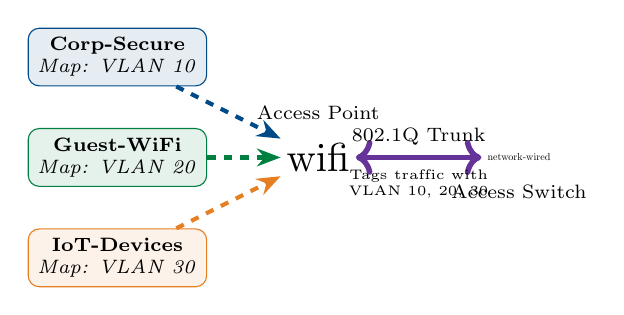
\begin{tikzpicture}[scale=0.85]
                    \node[wifi] (ap) at (0,0) {\iconwifi[0.8cm]};
                    \node[font=\scriptsize, above=0.1cm of ap] {Access Point};
                    
                    \node[font=\scriptsize, align=center, fill=rctcblue!10, rounded corners, draw=rctcblue] (ssid1) at (-3, 1.5) {\textbf{Corp-Secure} \\ \textit{Map: VLAN 10}};
                    \node[font=\scriptsize, align=center, fill=networkgreen!10, rounded corners, draw=networkgreen] (ssid2) at (-3, 0) {\textbf{Guest-WiFi} \\ \textit{Map: VLAN 20}};
                    \node[font=\scriptsize, align=center, fill=aborange!10, rounded corners, draw=aborange] (ssid3) at (-3, -1.5) {\textbf{IoT-Devices} \\ \textit{Map: VLAN 30}};
                    
                    \node[switch] (sw) at (3,0) {\iconswitch[0.8cm]};
                    \node[font=\scriptsize, align=center, below=0.1cm of sw] {Access Switch};
                    
                    \draw[wireless, dashed, rctcblue] (ssid1) -- (ap);
                    \draw[wireless, dashed, networkgreen] (ssid2) -- (ap);
                    \draw[wireless, dashed, aborange] (ssid3) -- (ap);
                    
                    \draw[trunk, <->] (ap) -- (sw) node[midway, above, font=\scriptsize] {802.1Q Trunk};
                    \node[font=\tiny, align=center] at (1.5, -0.4) {Tags traffic with\\VLAN 10, 20, 30};
                \end{tikzpicture}
            \end{center}
        \end{column}
    \end{columns}
\end{frame}

% =============================================================================
% SLIDE 21: AUTONOMOUS VS LIGHTWEIGHT
% =============================================================================
\begin{frame}{Autonomous vs. Lightweight Architecture}
    \begin{columns}[T]
        \begin{column}{0.48\textwidth}
            \begin{block}{Autonomous APs (Fat APs)}
                \begin{itemize}
                    \item Standalone, self-contained devices (like a standard home router).
                    \item Each AP contains its own management, security protocols, routing intelligence, and QoS rules.
                    \item \textbf{The Scaling Problem:} If an enterprise has 500 APs, a password change or firmware update requires logging into 500 separate management interfaces. \emph{It does not scale.}
                \end{itemize}
            \end{block}
        \end{column}
        \begin{column}{0.48\textwidth}
            \begin{block}{Lightweight APs (Thin APs)}
                \begin{itemize}
                    \item Stripped-down radios that do little more than broadcast RF and forward frames.
                    \item All "brains" (authentication, roaming decisions, channel assignments, security) are moved to a centralized \keyterm{Wireless LAN Controller (WLC)}.
                    \item \textbf{The Solution:} You configure the WLC once, and it pushes the configuration dynamically to all 500 APs instantly.
                \end{itemize}
            \end{block}
        \end{column}
    \end{columns}
\end{frame}

% =============================================================================
% SLIDE 22: WLC AND CAPWAP
% =============================================================================
\begin{frame}{The WLC and CAPWAP Tunnels}
    \begin{columns}[T]
        \begin{column}{0.5\textwidth}
            \begin{itemize}
                \item Lightweight APs communicate with the WLC using \keyterm{CAPWAP} (Control and Provisioning of Wireless Access Points), UDP ports 5246/5247.
                \item \textbf{Split-MAC Architecture:} 
                    \begin{itemize}
                        \item \textbf{AP handles real-time tasks:} Beacons, ACKs, and RF transmission.
                        \item \textbf{WLC handles management:} Authentication, roaming, and security.
                    \end{itemize}
                \item \textbf{Data Tunneling:} In most enterprise designs, all user Wi-Fi traffic is tunneled directly to the WLC before being dropped onto the wired LAN.
            \end{itemize}
        \end{column}
        \begin{column}{0.48\textwidth}
            \begin{center}
                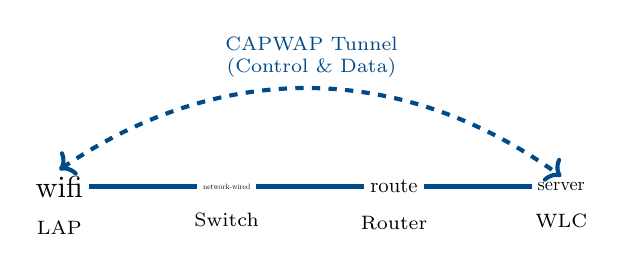
\begin{tikzpicture}[scale=0.85]
                    \node[wifi] (ap) at (0,0) {\iconwifi[0.6cm]};
                    \node[font=\scriptsize, below=0.1cm of ap] {LAP};
                    
                    \node[switch] (sw1) at (2.5,0) {\iconswitch[0.6cm]};
                    \node[font=\scriptsize, below=0.1cm of sw1] {Switch};
                    
                    \node[router] (rt) at (5,0) {\iconrouter[0.6cm]};
                    \node[font=\scriptsize, below=0.1cm of rt] {Router};
                    
                    \node[server] (wlc) at (7.5,0) {\iconserver[0.6cm]};
                    \node[font=\scriptsize, below=0.1cm of wlc] {WLC};
                    
                    % Physical Connections
                    \draw[ethernet noarrow] (ap) -- (sw1);
                    \draw[ethernet noarrow] (sw1) -- (rt);
                    \draw[ethernet noarrow] (rt) -- (wlc);
                    
                    % CAPWAP Tunnel
                    \draw[rctcblue, dashed, line width=1.5pt, bend left=35, <->] 
                        (ap.north) to node[above, font=\scriptsize, align=center] {CAPWAP Tunnel\\(Control \& Data)} (wlc.north);
                \end{tikzpicture}
            \end{center}
            \vspace{0.2em}
            \begin{alertblock}{Design Note}
                Because all traffic flows through the WLC, the WLC must be placed at a high-bandwidth choke point (like the Core or Data Center).
            \end{alertblock}
        \end{column}
    \end{columns}
\end{frame}

% =============================================================================
% SLIDE 23: SITE SURVEYS
% =============================================================================
\begin{frame}{Physical Design: The Site Survey}
    \begin{itemize}
        \item A \keyterm{Site Survey} is the critical process of planning AP placement to ensure adequate coverage, capacity, and minimal interference.
    \end{itemize}
    
    \vspace{0.3em}
    \begin{columns}[T]
        \begin{column}{0.32\textwidth}
            \begin{block}{Predictive Survey}
                \footnotesize
                Performed off-site using CAD floorplans and RF simulation software (e.g., Ekahau). Walls are drawn and assigned attenuation values (brick vs. drywall) to mathematically estimate AP coverage.
            \end{block}
        \end{column}
        \begin{column}{0.32\textwidth}
            \begin{block}{Active Survey}
                \footnotesize
                An engineer walks the actual building with a testing laptop, actively connecting to test APs ("AP on a stick") to measure real-world throughput, latency, and packet loss.
            \end{block}
        \end{column}
        \begin{column}{0.32\textwidth}
            \begin{block}{Passive Survey}
                \footnotesize
                Walking the building with a spectrum analyzer purely to listen. Used to map existing RF noise, detect rogue APs, and identify non-Wi-Fi interference (microwaves, Bluetooth).
            \end{block}
        \end{column}
    \end{columns}
\end{frame}

% =============================================================================
% SLIDE 24: ANTENNAS & ROAMING
% =============================================================================
\begin{frame}[shrink=10]{Antenna Types and Coverage Cells}
    \begin{columns}[T]
        \begin{column}{0.5\textwidth}
            \begin{itemize}
                \item \keyterm{Omnidirectional (Dipole):} Radiates RF energy equally in a 360-degree donut shape. Ideal for ceiling mounts in the center of standard rooms.
                \item \keyterm{Directional (Patch/Yagi):} Focuses RF energy in a specific direction, increasing gain (reach) in that direction while reducing it elsewhere. Ideal for long hallways, high warehouse ceilings, or bridging buildings.
            \end{itemize}
            
            \vspace{0.3em}
            \begin{exampleblock}{Seamless Roaming}
                As a user walks, their device must seamlessly \keyterm{roam} from AP 1 to AP 2. This requires exactly \textbf{15\% to 20\% coverage overlap} between the RF cells.
            \end{exampleblock}
        \end{column}
        \begin{column}{0.48\textwidth}
            \begin{center}
                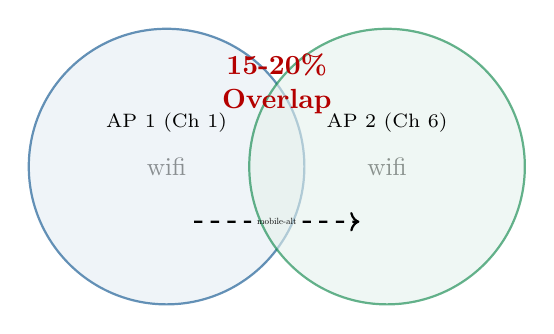
\begin{tikzpicture}[scale=0.7]
                    % AP 1 and Cell
                    \node[wifi] (ap1) at (0,0) {\iconwifi[0.5cm]};
                    \draw[thick, rctcblue, fill=rctcblue!10, opacity=0.6] (0,0) circle (2.5cm);
                    \node[font=\scriptsize] at (0, 0.8) {AP 1 (Ch 1)};
                    
                    % AP 2 and Cell
                    \node[wifi] (ap2) at (4,0) {\iconwifi[0.5cm]};
                    \draw[thick, networkgreen, fill=networkgreen!10, opacity=0.6] (4,0) circle (2.5cm);
                    \node[font=\scriptsize] at (4, 0.8) {AP 2 (Ch 6)};
                    
                    % Roaming user
                    \node[phone] (user) at (2, -1) {\iconphone[0.5cm]};
                    \draw[->, thick, dashed] (0.5, -1) -- (user) -- (3.5, -1);
                    
                    % Overlap label
                    \node[font=\scriptsize, align=center, text=alertred, font=\bfseries] at (2, 1.5) {15-20\%\\Overlap};
                \end{tikzpicture}
            \end{center}
            \vspace{0.2em}
            \scriptsize \textit{Note:} Adjacent APs must operate on non-overlapping channels. For 2.4 GHz, use 1 and 6 to prevent ACI in the roaming zone.
        \end{column}
    \end{columns}
\end{frame}

% =============================================================================
% SLIDE 25: CASE STUDY 2 SCENARIO
% =============================================================================
\begin{frame}[shrink=5]{Case Study: Robin's Starcourt Site Survey}
    \begin{casestudy}{The Food Court Dilemma}
        Robin Buckley is designing the AP layout for Starcourt Mall.
        She needs dense coverage for the food court and must keep the back-office signal from bleeding into the parking lot.
    \end{casestudy}
    
    \begin{block}{Review Questions}
        \begin{enumerate}
            \item For the dense food court, should Robin use a few high-powered APs or many low-powered APs? Why?
            \item What specific type of antenna should Robin deploy near the glass doors to stop the signal from bleeding into the parking lot?
        \end{enumerate}
    \end{block}
\end{frame}

% =============================================================================
% SLIDE 26: CASE STUDY 2 SOLUTION
% =============================================================================
\begin{frame}[shrink=5]{Case Study Solution: Robin's Starcourt Site Survey}
    \begin{casesolution}{The Food Court Dilemma}
        \begin{enumerate}
            \item \textbf{Food Court Density:} She should deploy \textbf{many low-powered APs}. High-powered APs create massive coverage cells, forcing hundreds of devices to fight for airtime on a single channel (a CSMA/CA nightmare). Small, low-power cells (Microcells) allow Robin to reuse channels, dramatically increasing total bandwidth capacity.
            \item \textbf{Parking Lot Bleed:} Robin should use \textbf{Directional (Patch) antennas} mounted on the interior perimeter walls, aimed \emph{inward} toward the mall. Standard omnidirectional antennas would radiate 360 degrees, sending half their RF energy straight through the glass into the parking lot.
        \end{enumerate}
    \end{casesolution}
    
    \begin{alertblock}{Key Takeaway}
        Good wireless design isn't about making the signal as loud as possible; it is about strictly controlling the shape, size, and boundaries of the RF cell.
    \end{alertblock}
\end{frame}

% =============================================================================
% SLIDE 27: SECTION 4 INTRO
% =============================================================================
\begin{frame}
    \begin{center}
        \Huge \textbf{Section 4}\\
        \vspace{0.5em}
        \Large \textcolor{rctcblue}{Wireless Security \& Access}
    \end{center}
\end{frame}

% =============================================================================
% SLIDE 28: ENCRYPTION PROTOCOLS
% =============================================================================
\begin{frame}{The Evolution of Wireless Encryption}
    \begin{itemize}
        \item RF data is broadcasted in open air. Without encryption, anyone with a protocol analyzer (like Wireshark) can capture and read all network traffic.
    \end{itemize}
    
    \vspace{0.3em}
    \begin{table}[]
        \renewcommand{\arraystretch}{1.5}
        \centering
        \scriptsize
        \resizebox{\textwidth}{!}{%
        \begin{tabular}{|l|l|l|l|}
        \hline
        \rowcolor[HTML]{EFEFEF} \textbf{Protocol} & \textbf{Cipher / Encryption} & \textbf{Key Vulnerability} & \textbf{Modern Status} \\ \hline
        \textbf{WEP} & RC4 (Weak 24-bit IVs) & IVs repeat; can be cracked in minutes by capturing traffic. & \textbf{Dead.} Never use under any circumstance. \\ \hline
        \textbf{WPA} & TKIP (RC4 wrapper) & Band-aid fix designed to run on old WEP hardware. & \textbf{Deprecated.} Easily compromised. \\ \hline
        \textbf{WPA2} & \textbf{AES / CCMP} & Dictionary/Brute-force attacks against the Pre-Shared Key (4-way handshake). & \textbf{Current Standard.} Secure if the password is long/complex. \\ \hline
        \textbf{WPA3} & \textbf{AES / GCMP} & None widely known yet. Uses \textbf{SAE} instead of PSK. & \textbf{The Future.} Mandatory for Wi-Fi 6E (6 GHz). \\ \hline
        \end{tabular}
        }
    \end{table}
    
    \begin{alertblock}{WPA3 and Forward Secrecy}
        WPA3's SAE (Simultaneous Authentication of Equals) provides \keyterm{Forward Secrecy}. If an attacker records encrypted Wi-Fi traffic today, and steals the password tomorrow, they \emph{still} cannot decrypt the old traffic.
    \end{alertblock}
\end{frame}

% =============================================================================
% SLIDE 29: PERSONAL VS ENTERPRISE
% =============================================================================
\begin{frame}{Authentication: Personal vs. Enterprise}
    \begin{columns}[T]
        \begin{column}{0.48\textwidth}
            \begin{block}{WPA2 / WPA3 - Personal (PSK)}
                \begin{itemize}
                    \item Uses a \keyterm{Pre-Shared Key} (password).
                    \item Every single device on the network types in the exact same password.
                    \item \textbf{The Fatal Flaw for Business:} If an employee is fired, you must change the Wi-Fi password on \emph{every single device} in the company to properly revoke their access.
                    \item Suitable only for homes and small coffee shops.
                \end{itemize}
            \end{block}
        \end{column}
        \begin{column}{0.48\textwidth}
            \begin{block}{WPA2 / WPA3 - Enterprise (802.1X)}
                \begin{itemize}
                    \item Uses \keyterm{802.1X} and a back-end \textbf{RADIUS} server (tied to Active Directory).
                    \item Users authenticate with their own unique username/password, or a digital certificate.
                    \item \textbf{The Enterprise Benefit:} If someone is fired, you disable their specific AD account. Their Wi-Fi access is instantly revoked, and nobody else is affected.
                \end{itemize}
            \end{block}
        \end{column}
    \end{columns}
\end{frame}

% =============================================================================
% SLIDE 30: BYOD AND CAPTIVE PORTALS
% =============================================================================
\begin{frame}{Managing Guest Access and BYOD}
    \begin{columns}[T]
        \begin{column}{0.52\textwidth}
            \begin{itemize}
                \item \keyterm{BYOD (Bring Your Own Device)} policies allow employees to use personal smartphones. Because IT does not control these devices, they must be treated as untrusted (placed on an isolated VLAN).
                \item \keyterm{MDM (Mobile Device Management)}: Software profiles installed on personal devices that enforce security policies (PIN required, encrypted storage) before granting access to corporate Wi-Fi and email.
            \end{itemize}
        \end{column}
        \begin{column}{0.45\textwidth}
            \begin{block}{Captive Portals}
                \begin{itemize}
                    \item A web page that intercepts HTTP/DNS traffic until a user completes an action.
                    \item Used to enforce an \textbf{Acceptable Use Policy (AUP)}, process payments, or verify an email address.
                    \item \textbf{Warning:} Networks with Captive Portals are typically \textbf{Open} (no Layer 2 encryption). Traffic can be intercepted easily.
                \end{itemize}
            \end{block}
        \end{column}
    \end{columns}
\end{frame}

% =============================================================================
% SLIDE 31: ROGUE APS AND EVIL TWINS
% =============================================================================
\begin{frame}[shrink=10]{Wireless Threats: Rogue APs and Evil Twins}
    \begin{columns}[T]
        \begin{column}{0.5\textwidth}
            \begin{block}{Rogue Access Point}
                \begin{itemize}
                    \item Unauthorized AP plugged into the corporate network.
                    \item Often installed by an employee for convenience.
                    \item \textbf{Danger:} Bypasses firewall, RADIUS, and WLC.
                \end{itemize}
            \end{block}
            \begin{block}{Evil Twin Attack}
                \begin{itemize}
                    \item Malicious AP spoofing the legitimate corporate SSID.
                    \item Devices roam to the strongest signal, letting the attacker intercept traffic.
                \end{itemize}
            \end{block}
        \end{column}
        \begin{column}{0.48\textwidth}
            \begin{center}
                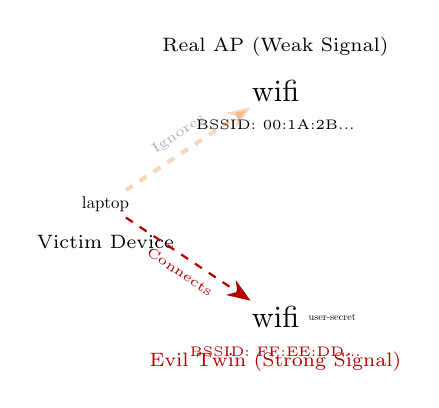
\begin{tikzpicture}[scale=0.72]
                    \node[pc] (victim) at (0,0) {\iconlaptop[0.6cm]};
                    \node[font=\scriptsize, below=0.1cm of victim] {Victim Device};
                    
                    \node[wifi] (real) at (3,2) {\iconwifi[0.6cm]};
                    \node[font=\scriptsize, above=0.1cm of real] {Real AP (Weak Signal)};
                    \node[font=\tiny] at (3, 1.4) {BSSID: 00:1A:2B...};
                    
                    \node[wifi] (evil) at (3,-2) {\iconwifi[0.6cm]};
                    \node[font=\scriptsize, below=0.1cm of evil, alertred] {Evil Twin (Strong Signal)};
                    \node[font=\tiny, alertred] at (3, -2.6) {BSSID: FF:EE:DD...};
                    \node at (4,-2) {\iconhacker[0.6cm]};
                    
                    \draw[wireless, opacity=0.3] (victim) -- node[above, sloped, font=\tiny] {Ignores} (real);
                    \draw[wireless, alertred, thick] (victim) -- node[below, sloped, font=\tiny, text=alertred] {Connects} (evil);
                \end{tikzpicture}
            \end{center}
            \vspace{0.2em}
            \begin{alertblock}{Defense}
                Use a \keyterm{WIDS/WIPS} to scan for spoofed MAC addresses and unauthorized APs.
            \end{alertblock}
        \end{column}
    \end{columns}
\end{frame}

% =============================================================================
% SLIDE 32: CASE STUDY 3 SCENARIO
% =============================================================================
\begin{frame}[shrink=5]{Case Study: Steve's Evil Twin}
    \begin{casestudy}{The Stolen Credentials}
        Steve Harrington sees staff phones connect to an open guest network named "Starcourt\_Staff" with a captive portal.
        A second AP with the same SSID is sitting in a van outside the breakroom and blasting a much stronger signal.
    \end{casestudy}
    
    \begin{block}{Review Questions}
        \begin{enumerate}
            \item What specific type of attack is the van in the parking lot executing?
            \item Why are the employee's personal phones automatically connecting to the van's AP instead of the real one inside the mall?
            \item How would moving to \textbf{WPA2-Enterprise (802.1X)} instead of an Open Captive Portal prevent this attack?
        \end{enumerate}
    \end{block}
\end{frame}

% =============================================================================
% SLIDE 33: CASE STUDY 3 SOLUTION
% =============================================================================
\begin{frame}[shrink=5]{Case Study Solution: Steve's Evil Twin}
    \begin{casesolution}{The Stolen Credentials}
        \begin{enumerate}
            \item \textbf{Evil Twin:} The attacker in the van is spoofing the legitimate network name and serving a fake Captive Portal page to harvest credentials.
            \item \textbf{Signal Strength / Roaming:} Wireless client drivers are programmed to aggressively roam to the AP with the strongest RF signal. Because the van is pumping out high power near the breakroom, the phones switch to it automatically.
            \item \textbf{802.1X Mutual Authentication:} If the network used 802.1X (EAP-TLS or PEAP), the authentication process requires mutual trust. The employee's phone would challenge the van's AP to present a valid digital certificate signed by the corporate CA. Because the van doesn't have it, the phone silently aborts the connection, keeping the credentials safe.
        \end{enumerate}
    \end{casesolution}
    
    \begin{alertblock}{Key Takeaway}
        Open networks with Captive Portals are trivial to spoof and provide no Layer 2 encryption. 802.1X secures BYOD access by cryptographically verifying both the user \emph{and} the network infrastructure.
    \end{alertblock}
\end{frame}

% =============================================================================
% SLIDE 34: SECTION 5 INTRO
% =============================================================================
\begin{frame}
    \begin{center}
        \Huge \textbf{Section 5}\\
        \vspace{0.5em}
        \Large \textcolor{rctcblue}{Wireless Troubleshooting}
    \end{center}
\end{frame}

% =============================================================================
% SLIDE 35: ENVIRONMENTAL ISSUES
% =============================================================================
\begin{frame}[shrink=5]{Environmental Issues and RF Attenuation}
    \begin{columns}[T]
        \begin{column}{0.5\textwidth}
            \begin{itemize}
                \item When troubleshooting wireless coverage gaps, the physical environment is the primary suspect.
                \item \keyterm{Attenuation}: The natural loss of signal strength as an RF wave travels through space or passes through materials.
            \end{itemize}
            
            \vspace{0.3em}
            \begin{block}{RF Behaviors}
                \begin{itemize}
                    \footnotesize
                    \item \textbf{Absorption:} Materials (concrete, brick, human bodies) absorb RF energy, killing the signal.
                    \item \textbf{Reflection:} Metal objects (filing cabinets, elevator shafts) bounce the signal, causing multipath interference.
                    \item \textbf{Refraction:} Glass and water can bend the RF wave, changing its trajectory.
                \end{itemize}
            \end{block}
        \end{column}
        \begin{column}{0.48\textwidth}
            \begin{alertblock}{Non-Wi-Fi Interference}
                \begin{itemize}
                    \footnotesize
                    \item Wi-Fi runs in unlicensed ISM bands. 
                    \item Baby monitors, microwaves, cordless phones, and Bluetooth all share the 2.4 GHz band.
                    \item Because CSMA/CA requires devices to wait for "clear air", non-Wi-Fi interference doesn't just corrupt data—it freezes the channel completely.
                \end{itemize}
            \end{alertblock}
            \begin{exampleblock}{The Rule of 3s and 10s (dB)}
                In RF math:
                \begin{itemize}
                    \item $+3$ dB doubles the power.
                    \item $-3$ dB halves the power.
                    \item $+10$ dB increases power by 10x.
                \end{itemize}
            \end{exampleblock}
        \end{column}
    \end{columns}
\end{frame}

% =============================================================================
% SLIDE 36: SIGNAL METRICS (RSSI AND SNR)
% =============================================================================
\begin{frame}[shrink=5]{Troubleshooting Metrics: RSSI and SNR}
    \begin{columns}[T]
        \begin{column}{0.5\textwidth}
            \begin{itemize}
                \item \keyterm{RSSI (Received Signal Strength Indicator):} A measurement of how well your device can hear the AP. Measured in \textbf{negative dBm}.
                \item Closer to zero is better.
                \item \keyterm{Noise Floor:} The background ambient RF noise (microwaves, cosmic radiation, neighbor's Wi-Fi).
                \item \keyterm{SNR (Signal-to-Noise Ratio):} The difference between the RSSI and the Noise Floor. A high SNR means the signal is clearly distinguishable from the noise.
            \end{itemize}
        \end{column}
        \begin{column}{0.48\textwidth}
            \begin{table}[]
                \renewcommand{\arraystretch}{1.3}
                \centering
                \scriptsize
                \resizebox{\linewidth}{!}{%
                \begin{tabular}{|l|l|}
                \hline
                \rowcolor[HTML]{EFEFEF} \textbf{RSSI Value} & \textbf{Expected Performance} \\ \hline
                \textbf{-30 dBm} & Perfect (Right next to AP) \\ \hline
                \textbf{-65 dBm} & Excellent (Enterprise standard) \\ \hline
                \textbf{-70 dBm} & Good (Reliable packet delivery) \\ \hline
                \textbf{-80 dBm} & Poor (Dropped packets, slow) \\ \hline
                \textbf{-90 dBm} & Unusable (Disconnects) \\ \hline
                \end{tabular}
                }
            \end{table}
            
            \vspace{0.3em}
            \begin{exampleblock}{Calculating SNR}
                Signal: $-65$ dBm \\
                Noise Floor: $-90$ dBm \\
                SNR = $25$ dB (\textit{Excellent})
                \\ \vspace{0.2em}
                \scriptsize *If SNR drops below $10$ dB, the device cannot decode the transmission.
            \end{exampleblock}
        \end{column}
    \end{columns}
\end{frame}

% =============================================================================
% SLIDE 37: COMMON CONFIG ISSUES
% =============================================================================
\begin{frame}[shrink=5]{Common Configuration and Placement Issues}
    \begin{columns}[T]
        \begin{column}{0.48\textwidth}
            \begin{block}{Improper AP Placement}
                \begin{itemize}
                    \item \textbf{Too High:} Mounting APs on 30-foot warehouse ceilings puts clients too far away.
                    \item \textbf{Hidden APs:} Placing APs above drop ceilings near metal HVAC ducts severely attenuates and reflects the signal.
                    \item \textbf{Wall Mounts:} Mounting omnidirectional APs sideways on a wall instead of flat on a ceiling pushes half the signal into the floor/ceiling.
                \end{itemize}
            \end{block}
        \end{column}
        \begin{column}{0.48\textwidth}
            \begin{block}{Logical Configuration Errors}
                \begin{itemize}
                    \item \textbf{Channel Overlap:} Manually assigning an AP to Channel 3 on the 2.4 GHz band causes crippling Adjacent Channel Interference.
                    \item \textbf{Capacity Overload:} Connecting 100 students to a single AP in an auditorium. Wi-Fi is shared; airtime becomes exhausted.
                    \item \textbf{Frequency Mismatch:} A legacy 2.4 GHz IoT device cannot see an SSID that is only broadcasting on 5 GHz.
                \end{itemize}
            \end{block}
        \end{column}
    \end{columns}
\end{frame}

% =============================================================================
% SLIDE 38: CASE STUDY 4 SCENARIO
% =============================================================================
\begin{frame}[shrink=5]{Case Study: Hopper's Microwave Mystery}
    \begin{casestudy}{The Lunchtime Latency}
        Jim Hopper, IT Director at the Hawkins Police Station, is aggressively troubleshooting a massive latency spike that happens every day exactly at 12:30 PM on the dispatch floor. 
        
        \vspace{0.5em}
        During this window, wireless IP phones drop calls, and the dispatch software running on 2.4 GHz laptops disconnects entirely. Checking the WLC logs, Hopper sees that the AP serving the dispatch floor is experiencing 90\% channel utilization and massive packet retries, despite only having 5 connected devices.
    \end{casestudy}
    
    \begin{block}{Review Questions}
        \begin{enumerate}
            \item What phenomenon is occurring every day at 12:30 PM?
            \item Why does this non-Wi-Fi interference cause Wi-Fi packet retries and high channel utilization?
            \item What are two potential solutions Hopper can implement to fix the dispatch network?
        \end{enumerate}
    \end{block}
\end{frame}

% =============================================================================
% SLIDE 39: CASE STUDY 4 SOLUTION
% =============================================================================
\begin{frame}[shrink=5]{Case Study Solution: Hopper's Microwave Mystery}
    \begin{casesolution}{The Lunchtime Latency}
        \begin{enumerate}
            \item \textbf{Non-Wi-Fi Interference:} Joyce is heating up her lunch. Microwave ovens operate at 2.4 GHz. A leaky, unshielded microwave acts as a massive RF jammer on the 2.4 GHz band.
            \item \textbf{CSMA/CA Breakdown:} Wi-Fi devices must perform a Clear Channel Assessment (CCA). When the microwave is running, the channel is never clear. Devices wait indefinitely (latency). When they do try to transmit, the RF noise corrupts the frame, no ACK is received, and the packet must be retried.
            \item \textbf{Solutions:} 
                \begin{itemize}
                    \item \textit{Solution A:} Move the dispatch laptops and IP phones to the \textbf{5 GHz band}, completely avoiding the microwave's frequency.
                    \item \textit{Solution B:} Throw the leaky microwave away and buy a properly shielded one for the breakroom.
                \end{itemize}
        \end{enumerate}
    \end{casesolution}
\end{frame}

% =============================================================================
% SLIDE 40: MODULE SUMMARY
% =============================================================================
\begin{frame}[shrink=5]{Module 12.0 Summary}
    \begin{columns}[T]
        \begin{column}{0.48\textwidth}
            \begin{block}{Wireless Fundamentals}
                \begin{itemize}
                    \item RF uses 2.4 GHz (range/crowded), 5 GHz (speed/clean), and 6 GHz (Wi-Fi 6E/7).
                    \item Wi-Fi uses CSMA/CA to avoid collisions.
                    \item 802.11 evolved from DSSS (802.11b) to MIMO (802.11n) to OFDMA (802.11ax).
                \end{itemize}
            \end{block}
            
            \vspace{0.3em}
            \begin{block}{Enterprise Design}
                \begin{itemize}
                    \item WLCs manage lightweight APs via CAPWAP tunnels for centralized control.
                    \item Antenna choice (Omni vs. Directional) shapes the RF cell to optimize coverage.
                \end{itemize}
            \end{block}
        \end{column}
        \begin{column}{0.48\textwidth}
            \begin{block}{Security \& Threats}
                \begin{itemize}
                    \item WPA3 uses SAE for forward secrecy.
                    \item 802.1X (Enterprise) ties access to identity.
                    \item Rogue APs bypass firewalls; Evil Twins spoof real networks to steal credentials.
                    \item BYOD requires MDM or isolated VLANs.
                \end{itemize}
            \end{block}
            
            \vspace{0.3em}
            \begin{block}{Troubleshooting}
                \begin{itemize}
                    \item Good RSSI (-65 dBm) and high SNR are critical.
                    \item Non-Wi-Fi interference destroys 2.4 GHz.
                    \item Only use channels 1, 6, and 11 on 2.4 GHz.
                \end{itemize}
            \end{block}
        \end{column}
    \end{columns}
\end{frame}


\end{document}